\section{Základní pojmy z planimetrie, rovinné útvary, úhly v nich}
\begin{definition}
  Nechť $A,B,C\in \mathbb E_2$ jsou tři body. Jestliže všechny tři leží (resp. neleží) na jedné přímce, řekneme, že jsou \textbf{kolineární} (resp. \textbf{nekolineární}).
\end{definition}

\begin{definition}
  Nechť $p,q\in \mathscr P$. Jestliže platí:
  \begin{enumerate}[$i.$]
    \item $p=q$, pak přímky $p,q$ se nazývají \textbf{splývající rovnoběžky},
    \item $p \ne q \land p\cap q = \emptyset$, pak přímky $p,q$ se nazývají \textbf{různé rovnoběžky},
    \item $p \ne q \land p\cap q \ne \emptyset$, pak přímky $p,q$ se nazývají \textbf{různoběžky}.
  \end{enumerate}
\end{definition}

\begin{definition}
  Nechť $p\in \mathscr P,A \in p, B \in p, A \ne B.$ Množinu
  \[
    P(A)=\left \{ X\in \mathbb E_2; X=B \lor X\,\mu\, AB \lor B\, \mu\, AX \right \}
  \]
  (resp. množinu $P(A)\cup \{A\}$) nazýváme \textbf{otevřenou} (resp. \textbf{uzavřenou}) \textbf{polopřímkou} $AB$ s počátkem v bodě $A$. Množinu
  \[
    Q(A)=\left \{ X\in \mathbb E_2; A\,\mu\, BX \right \}
  \]
  (resp. množinu $Q(A)\cup \{A\}$) nazýváme \textbf{otevřenou} (resp. \textbf{uzavřenou}) \textbf{polopřímku opačnou} k polopřímce $AB$ s počátkem $A$.
\end{definition}

\begin{definition}
  Nechť body $A,B\in \mathbb E_2, A\ne B$. Průnik uzanřených polopřímek $AB$ a $BA$ nazveme \textbf{úsečkou} $AB$. Body $A,B$ se nazývají \textbf{krajní body úsečky} $AB$, bod $X\,\mu \, AB$ se nazývá \textbf{vnitřní bod} úsečky $AB$.
\end{definition}

\begin{definition}
Nechť $a\in \mathscr P, A\notin a, B\notin a, A\ne B.$ Pak \textbf{přímka} $a$ \textbf{odděluje body} $A,B$ a zapisujeme $a\, \nu\, AB.$ V opčaném případě \textbf{přímka} $a$ \textbf{neodděluje body} $A,B$. Zapisujeme $a\, \overline \nu \,AB.$
\end{definition}

\begin{definition}
  Nechť $a \in \mathscr P$. Pak všechny $X\in \mathbb E_2 - a$ lze rozdělit do dvou podmnožin $P(a), Q(a)$ tak, že:
  \begin{enumerate}[$i.$]
    \item přímka $a$ odděluje každé dva body z různých podmnožin:
      \[
        \forall x \in P(a), \forall Y \in Q(a): a \, \nu \, XY
      \]
    \item přímka $a$ neodděluje žádné dva body z jedné podmnožiny
      \[
        \forall X, Y \in P(a) \land \forall X,Y \in Q(a): a \,\overline \nu\, XY.
      \]
  \end{enumerate}
  Pak množinu $P(a)$ (resp. množinu $Q(a)$) nazveme \textbf{otevřenou polorovinou s hraniční přímkou} $a$ (resp. \textbf{otevřenou polorovinou s hraniční přímkou} $a$ \textbf{opačnou k} $P(a)$). Množinu $P(a)\cup a$ (resp. $Q(a) \cup a$) nazveme \textbf{uzavřenou polorovinou s hraniční přímkou} $a$ (resp. \textbf{uzavřenou polorovinou s hraniční přímkou} $a$ \textbf{opačnou k} $P(a)$).
\end{definition}

\begin{definition}
  Nechť $A,B,V \in \mathbb E_2$ jsou tři různé nekolineární body. Průnik polorovin $VBA \cap VAB$ nazveme \textbf{konvexním úhlem} (zapisujeme $\sphericalangle BVA$), $V$ jeho \textbf{vrcholem}, polopřímky $VA, VB$ jeho \textbf{rameny}. \textbf{Nekonvexním úhlem} $BVA$ nazveme sjednocení polorovin opačných k polorovinám $VBA,VAB.$
\end{definition}

\begin{definition}
  Nechť $A,B,C\in \mathbb E_2$ jsou tři různé nekolineární body. \textbf{Trojúhelníkem} $ABC$ (značíme $\triangle ABC$) nazýváme průnik polorovin $\overrightarrow{ABC} \cap \overrightarrow{BCA} \cap \overrightarrow{CAB}$. Body $A,B,C$ nazýváme \textbf{vrcholy} tohoto trojúhelníka, úsečky $AB, BC, CA$ jeho \textbf{stranami}.
\end{definition}

\begin{definition}
  Nechť $A,B\in \mathbb E_2.$ Přiřaďme uspořádané dvojici bodů $(A,B)$ reálné číslo označené $|AB|,$ pro něž platí:
  \begin{enumerate}[$i.$]
    \item $|AB|\geq 0,$ přičemž $|AB|=0 \iff A=B,$
    \item $|AB|=|BA|,$
    \item $C\, \mu \, AB \implies |AB|=|CB|+|AC|,$
    \item nechť $AB$ je polopřímka, $m\in \mathbb R^+_0.$ Pak $\exists ! C\in AB$ tak, že $|AC|=m.$
  \end{enumerate}
\end{definition}

\begin{definition}
  Každému konvexnímu úhlu $\sphericalangle AVC$ přiřaďme \textbf{velikost úhlu} (ozn. $|\sphericalangle AVC|$) ve stupních tak, že
  \begin{enumerate}[$i.$]
    \item nulový úhel má velikost $0^\circ$, přímý $180^\circ$,
    \item každý jiný konvexní úhel má velikost $n^\circ, $ kde $0^\circ< n ^\circ< 180^\circ, u \in \mathbb R,$
    \item jestliže polopřímka $VB$ prochází mezi rameny konvexního úhlu $\sphericalangle AVC$, pak $|\sphericalangle AVC|=|\sphericalangle AVB|+ |\sphericalangle BVC|$ a
    \item nechť $VA$ je polopřímka, $u \in \mathbb R, u \in \left < 0 ^\circ,180^\circ \right >$. Pak existuje polopřímka $VB$ taková, že $|\sphericalangle AVB|=u^\circ.$
  \end{enumerate}
\end{definition}

\begin{pozn}
  \textbf{Radián} je středový úhel příslušný v jednotkové kružnici kruhovému oblouku délky 1. Z definice plyne:
  \[
    360^\circ = 2\pi.
  \]
\end{pozn}

\begin{definition}
  Nechť $p,q\in \mathscr P$ jsou dvě různoběžky. Řekneme, že $p,q$ jsou na sebe \textbf{kolmé} (a zapisujeme $p\perp q$), jestliže všechny čtyři úhly, které spolu svírají, jsou shodné (a tedy pravé).
\end{definition}

\begin{pozn}[Klasifikace úhlů podle velikosti]
  Nechť $\alpha$ je velikost úhlu $|\sphericalangle ABC|$. Potom je úhel $|\sphericalangle ABC|$
  \begin{itemize}
    \item nulový, pokud $\alpha=0^\circ$,
  \item ostrý, pokud $0^\circ <\alpha < 90^\circ,$
  \item pravý, pokud $\alpha = 90^\circ,$
  \item tupý, pokud $90^\circ < \alpha < 180^\circ,$
  \item přímý, pokud $\alpha = 180^\circ,$
  \item konvexní, pokud $0^\circ \leq \alpha \leq 180^\circ,$
  \item nekonvexní, pokud $180^\circ < \alpha < 360^\circ$,
  \item plný, pokud $\alpha = 360^\circ,$
  \item kosý, pokud je ostrý nebo tupý.
  \end{itemize}
\end{pozn}

\begin{definition}
  Nechť $A,B\in \mathbb E_2$. \textbf{Vzdáleností bodů} $A,B$ nazveme délku úsečky $AB.$
\end{definition}


\begin{definition}
  Nechť $P\in \mathbb E_2, p \in \mathscr P.$ \textbf{Vzdáleností bodu} $P$ \textbf{od přímky} $p$ nazveme reálné číslo označené $\rho(P,p)$ takové, že $\rho(P,p)=|PP_0|,$ kde $P_0$ je kolmý průmět bodu $p$ na přímku $p$.
\end{definition}

\begin{definition}
  Nechť $a,b \in \mathscr P, a \parallel b.$ \textbf{Vzdáleností dvou přímek} $a,b$ nazveme reálné číslo označené $\rho(a,b)$ takové, že $\rho(a,b)=\rho(A,b),$ kde $A\in a$ je libovolný bod.
\end{definition}

\begin{definition}
  Nechť $a,b\in \mathscr P.$ \textbf{Odchylkou přímek} $a,b$ nazveme reálné číslo $\varphi^\circ\in \left <0, 180\right>$, kde $\varphi$ je velikost úhlu, který spolu přímky $a,b$ svírají. U rovnoběžek klademe $\varphi = 0^\circ.$
\end{definition}

\begin{definition}
  Dvojice úhlů:
  \begin{itemize}
    \item \textbf{vrcholové úhly} -- dvojice úhlů, jejichž ramena jsou opačné polopřímky
    \item \textbf{vedlejší úhly} --	dvojice úhlů, jejichž jedno rameno je společné a druhá ramena jsou opačné polopřímky
    \item \textbf{souhlasné úhly} -- dvojice úhlů, jejichž první ramena leží na jedné přímce a druhá ramena jsou rovnoběžná, přitom směr příslušných ramen je stejný
    \item \textbf{střídavé úhly}	-- dvojice úhlů, jejichž první ramena leží na jedné přímce a druhá ramena jsou rovnoběžná, přitom směr příslušných ramen je opačný
    \item \textbf{přilehlé úhly} -- dvojice úhlů, jejichž první ramena leží na jedné přímce a jdou do opačných směrů a druhá ramena jsou rovnoběžná
  \end{itemize}
\end{definition}

\begin{definition}
  Dvě polopřímky, ležící na téže přímce nazýváme \textbf{souhlasnými}, jestliže jedna z nich je podmnožinou druhé. V opačném případě je nazveme \textbf{nesouhlasnými}.
\end{definition}

\begin{definition}
  Nechť $\triangle ABC$. \textbf{Vnitřním úhlem} $\triangle ABC$ při vrcholu $A$ ($B, C$) nazýváme $\sphericalangle CAB$ $(\sphericalangle ABC, \sphericalangle BCA)$, \textbf{vnějším úhlem} $\triangle ABC$ při vrcholu $A$ ($B, C$) pak vedlejší úhel k úhlu $\sphericalangle CAB$ ($\sphericalangle ABC, \sphericalangle BCA$).
\end{definition}

\begin{veta}
  Součet všech vnitřních úhlů v trojúhelníku je $180^\circ$.
\end{veta}

\begin{proof}
  $ $ \newline
  \begin{center}
   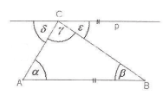
\includegraphics[width=0.5\linewidth]{trojuhelnik_1.png}
  \end{center}
\end{proof}

\begin{veta}
  Součet libovolných dvou vnitřních úhlů v trojúhelníku je menší něž $180^\circ$.
\end{veta}

\begin{proof}
  Plyne z předchozí věty a tvrzení, že vnitřní úhel v trojúhelníku je nenulový.
\end{proof}

\begin{veta}
  V každém trojúhelníku je velikost vnějšího úhlu při jednom vrcholu rovna součtu velikostí dvou zbylých vnitřních úhlů.
\end{veta}

\begin{proof}
  $$\alpha + \alpha^\prime = 180^\circ$$ (úhly vedlejší)
  $$\alpha + \beta + \gamma = 180^\circ$$
  $$\implies \alpha^\prime = \beta + \gamma\qedhere$$
\end{proof}

\begin{definition}
  Trojúhelník se nazývá \textbf{rovnoramenný}, jestliže alespoň dvě jeho strany jsou shodné úsečky. Strany stejné délky nazveme \textbf{rameny}, tu třetí \textbf{základnou} a vrchol proti základně \textbf{vrcholem}.
  Trojúhelník se nazývá \textbf{rovnostranný}, jestliže všechny tři jeho strany jsou shodné úsečky.
  Trojúhelník se nazývá \textbf{pravoúhlý}, jestliže je jeden jeho vnitřní úhel pravý. Dvě strany, které jsou rameny pravého úhlu nazveme \textbf{odvěsnami}, tu třetí \textbf{přeponou}.
\end{definition}

\begin{definition}
  \textbf{Střední příčkou} trojúhelníku nazýváme úsečku spojující středy dvou stran trojúhelníka.
  \textbf{Těžnicí} trojúhelníku nazýváme úsečku spojující vrchol trojúhelníku se středem protější strany.
  \textbf{Výškou} trojúhelníku nazýváme úsečku procházející vrcholem trojúhelníka, která je kolmá na přímku, na které leží protější strana trojúhelníku. Průsečík výšek nazýváme \textbf{ortocentrum}.
\end{definition}

\begin{veta}
  Každá střední příčka je rovnoběžná s protilehlou stranou a je dvakrát menší než protilehlá strana.
\end{veta}

\begin{proof}
  Trojúhelníky vrchol -- střední příčka a vrchol -- protilehlá strana jsou zjevně podobné s koeficientem 2.
\end{proof}

\begin{veta}
  Těžnice trojúhelníku se všechny protínají v jednom bodě, který je dělí v poměru $2:1$.
\end{veta}

\begin{proof}
    V trojúhelníku $ABC$ jsou těžnice $t_a,t_b,t_c$. Sestrojme body $X,Y$ tak, aby
    $ABXC$ a $ABCY$ byly rovnoběžníky. Jistě jsou $AX$, resp. $BY$ jejich úhlopříčky.
    Zároveň je $|AB|=|CX|=|CY|$, takže $C$ je střed $XY$. Těžnice $t_c$ je tím pádem
    osou souměrnosti lichoběžníka $ABXY$, a proto leží na průsečíku jeho úhlopříček
    (tento lichoběžník je rovnoramenný).\\
    V témže trojúhelníku označme středy stran $S_a,S_b,S_c$. Trojúhelník $S_aS_bS_c$ je
    pak podobný s trojúhelníkem $ABC$ s koeficientem $1/2$ (jeho strany jsou středními
    příčkami trojúhelníka $ABC$). Navíc těžnice \uv{menšího} trojúhelníka leží na
    těžnicích toho \uv{většího}. Proto i $|AT|=2|S_{S_bS_c}T|$, což jsme chtěli ukázat.
\end{proof}

\begin{definition}
Průsečík těžnic nazýváme \textbf{těžištěm}.
\end{definition}

\begin{veta}
  Nechť $\triangle ABC$ je rovnoramenný trojúhelník se základnou $AB$. Pak platí, že těžnice $t_c$ splývá s výškou $v_c$ a s osou úhlu $\sphericalangle ACB$.
\end{veta}

\begin{proof}
  Nechť $t_c = CC_1$, kde $C_1$ je středem $AB$.
  $\triangle AC_1 C \cong \triangle BC_1 C$ (sus), neboť $|AC| = |BC|, |AC_1| = |BC_1|$ a $|\sphericalangle CAC_1| = |\sphericalangle CBC_1|$
  \begin{enumerate}[$i.$]
    \item $|\sphericalangle AC_1 C| = |\sphericalangle BC_1 C| = 90^\circ \implies CC_1 = v_c$
    \item $|\sphericalangle AC_1 C| = |\sphericalangle BC_1 C| \implies CC_1 = $ osa úhlu $\sphericalangle ACB$\qedhere
  \end{enumerate}
\end{proof}

\begin{veta}[Trojúhelníková nerovnost]
  V každém $\triangle ABC$ platí, že součet délek dvou libovolných stran je větší než strana třetí.
\end{veta}

\begin{proof}
  Ukážeme, že $|AC| < |AB| + |BC|$. Sestrojme na $\overrightarrow{AB}$ bod $D$ tak, že $|BD| = |BC| \land B \mu AD$. $\triangle BCD$ je rovnoramenný s hlavním vrcholem B $\implies \omega_1 = \delta$
  $B \mu AD \implies \omega_1 < \omega$
  $\implies \delta < \omega \implies |AC| < |AD| = |AB| + |BD| = |AB| + |BC| \implies |AC| < |AB| + |BC|$
\end{proof}

\begin{veta}[Věty o shodnosti trojúhelníků]
  \begin{itemize}
    \item \textbf{sss}: Shodují-li se dva trojúhelníky ve všech třech odpovídajících si stranách, pak jsou shodné.
    \item \textbf{sus}: Shodují-li se dva trojúhelníky ve dvou stranách a úhlu jimi sevřeném, jsou shodné.
    \item \textbf{usu}: Shodují-li se dva trojúhelníky v jedné straně a v obou úhlech k ní přilehlých, jsou shodné.
    \item \textbf{Ssu}: Shodují-li se dva trojúhelníky ve dvou stranách a úhlu proti delší z nich, jsou shodné.
  \end{itemize}
\end{veta}

\begin{proof}
  Jednu si určím jako axiom (sus) a zbylé převedu na tuto rozkladem na případy.
\end{proof}

\begin{definition}
  Trojúhelníky jsou \textbf{podobné}, zapisujeme $\triangle ABC \approx \triangle DEF$, jestliže $\exists k \in \R^+:k = \frac{|AB|}{|DE|}=\frac{|BC|}{|EF|}=\frac{|CA|}{|FD|}$. Číslo $k$ nazveme \textbf{koeficientem podobnosti}.
\end{definition}

\begin{veta}[Věty o podobnosti trojúhelníků]
  \begin{itemize}
    \item \textbf{uu}: Shodují-li se dva trojúhelníky ve dvou úhlech, jsou podobné.
    \item \textbf{sus}: Shodují-li se dva trojúhelníky v poměru dvou stran a úhlu jimi sevřeném, jsou podobné.
  \end{itemize}
\end{veta}

\begin{veta}[Euklidova věta o výšce]
  Nechť je dán pravoúhlý trojúhelník ABC s přeponou AB. Pak platí, že obsah čtverce nad výškou na přeponu je roven obsahu obdélníka o stranách rovných úsekům na přeponě oddělených touto výškou.
  $$v_c^2 = c_a \cdot c_b$$
\end{veta}

\begin{proof}
  $\triangle ACC_0 \approx \triangle CBC_0$ (uu), neboť $\sphericalangle C_0 CB$ je otočením $\sphericalangle C_0 AC$
  $\frac{|CC_0|}{|AC_0|} = \frac{|BC_0|}{|CC_0|} \implies \frac{v_c}{c_b} = \frac{c_a}{v_c} \implies v_c^2 = c_a \cdot c_b$
\end{proof}

\begin{veta}[Euklidovy věty o odvěsnách]
  Nechť je dán pravoúhlý trojúhelník s přeponou AB. Pak platí, že obsah čtverce nad odvěsnou je roven obsahu obdélníka o stranách rovných přeponě a úseku na přeponě přilehlému k této odvěsně odděleného výškou na přeponu.
  \begin{align*}
    b^2 = c \cdot c_b\\
    a^2 = c \cdot c_a
  \end{align*}
\end{veta}

\begin{veta}[Pythagorova]
  Nechť je dán pravoúhlý trojúhelník $ABC$ s přeponou $c$. Pak
  \[
    a^2+b^2 = c^2.
  \]
\end{veta}


\begin{proof}
  Z Euklidovy věty o výšce platí $cc_a=a^2$, $cc_b=b^2$, po sečtení těchto dvou vztahů získáme
  \[
    cc_a+cc_b=a^2+b^2 \iff c(c_a+c_b)=a^2+b^2 \iff c^2=a^2+b^2. \qedhere
  \]
\end{proof}

blok čtyřúhelník a dál ---
\begin{definition}
  Nechť $A_1,A_2, A_3, A_4 \in \mathbb E_2$ jsou čtyři body, z nichž žádné tři nejsou kolineární. Sjednocení úseček $A_1A_2\cup A_2A_3 \cup A_3A_4 \cup A_4A_1$ nazveme \textbf{uzavřenou lomenou čárou}.
\end{definition}

\begin{definition}
  Nechť $ABCD$ je uzavřená lomená čára, která sama sebe neprotíná. Pak \textbf{čtyřúhelníkem} $ABCD$ nazveme sjednocení této lomené čáry s množinou jejích vnitřních bodů. Body $A,B,C,D$ se nazývají \textbf{vrcholy}, uzavřená lomená čára $ABCD$ \textbf{obvodem}, každá úsečka \textbf{stranou} a úsečky $AC,BD$ se nazývají \textbf{úhlopříčky}.
\end{definition}

\begin{veta}
  Součet vnitřních úhlů čtyřúhelníka je $360^\circ$.
\end{veta}

\begin{proof}
  --- insert obrázek //TODO % TODO
  $\delta+ \beta_1+ \alpha_2 = 180^\circ$\\
  $\gamma + \beta_2 + \alpha_1 = 180^\circ$\\
  $\alpha+\beta+\gamma+\delta=360^\circ$
\end{proof}

\begin{definition}
  Nechť $ABCD$ je čtyřúhelník, jehož protější strany jsou rovnoběžné. Pak ho nazveme \textbf{rovnoběžníkem}.
\end{definition}

\begin{veta}
  V rovnoběžníku $ABCD$ platí:
  \begin{enumerate}[$i.$]
    \item $|AB|=|CD| \land |BC|=|AD|,$
    \item protilehlé úhly jsou shodné.
  \end{enumerate}
\end{veta}

\begin{proof}
  Plyne ze shodnosti trojúhelníků $ABD$ a $CDB.$
\end{proof}

\begin{veta}
  Úhlopříčky rovnoběžníka se navzájem půlí.
\end{veta}


\begin{proof}
  Plyne ze shodnosti trojúhelníků $ASD$ a $CSB$, kde $S$ je průsečík úhlopříček.
\end{proof}

\begin{definition}
  Čtyřúhelník, jehož všechny čtyři úhly jsou pravé, nazveme \textbf{pravoúhelník}.
\end{definition}

\begin{veta}
  \begin{enumerate}[$i.$]
    \item Každý pravoúhelník je rovnoběžník.
    \item Úhlopříčky pravoúhelníka jsou shodné.
  \end{enumerate}
\end{veta}

\begin{proof}
  \begin{enumerate}[$i.$]
    \item Protější úhly v rovnoběžníku jsou střídavé úhly u rovnoběžek.
    \item Plyne ze shodnosti trojúhelníků $ABD$ a $BAC$.\qedhere
  \end{enumerate}
\end{proof}

\begin{definition}
  Rovnoběžník $ABCD$ se nazývá \textbf{kosočtvercem} (resp. \textbf{kosodélníkem}), jestliže $|AB|=|BC|$ (resp. $|AB\ne BC|$) a žádný vnitřní úhel není pravý.
\end{definition}


\begin{veta}
  Úhlopříčky v kosočtverci se navzájem půlí.
\end{veta}

\begin{definition}
  Pravoúhelník $ABCD$ nazýváme
  \begin{itemize}
    \item \textbf{čtvercem}, jestliže $|AB|=|BC|,$
    \item \textbf{obdélníkem}, jestliže $|AB| \ne |BC|$
  \end{itemize}
\end{definition}

\begin{definition}
  Konvexní čtyřúhelník $ABCD$, kde $AB \parallel CD \land BC \nparallel AD,$ nazveme \textbf{lichoběžníkem}. Strany $AB, CD$ nazveme \textbf{základnami} a strany $BC$ a $DA$ \textbf{rameny lichoběžníka}.
\end{definition}

\begin{definition}
  Uzavřená lomená čára $A_1A_2\dots A_nA_1$, která leží v rovině a sama sebe nikdy neprotíná ohraničuje část roviny, která se nazývá \textbf{mnohoúhelník} nebo také \textbf{$n$-úhelník}.
\end{definition}

blok kružnice, kruh, tětiva atd. ---
\begin{definition}
  Nechť $S \in \mathbb E_2, r \in \mathbb R^+.$\\
  \textbf{Kružnicí} (resp. \textbf{kruhem}) se středem $S$ a poloměrem $R$ nazýváme množinu všech bodů $X\in \mathbb E_2, $ kde $|SX|=r$ (resp. $|SX|\leq r$).
\end{definition}

\begin{definition}
  Nechť $k(S,r)$ je kružnice, $X_1, X_2 \in km X_1\ne X_2.$ Úsečku (resp. přímku) $X_1X_2$ nazýváme \textbf{tětivou} (resp. \textbf{sečnou}) kružnice $k$.
\end{definition}


\begin{definition}
  Nechť $k(S,r)$ je kružnice, $T\in k$. Přímku $t$, pro níž platí $T\in t \land ST \perp t$ nazýváme \textbf{tečnou} kružnice $k$ s \textbf{bodem dotyku} $T$.
\end{definition}

\begin{definition}
  Nechť je dán oblouk $AB$ na kružnici $k(S,r).$ Polopřímky $\overrightarrow{SA}, \overrightarrow{SB}$ jso urameny dvou úhlů, z nichž právě jedno obsahuje oblouk $AB$. Tento úhel nazýváme \textbf{středovým úhlem} příslušným oblouku $AB$. Každý úhel $\sphericalangle AXB,$ kde $X\in k \land X\in AB,$ nazýváme \textbf{obvodovým úhlem} příslušným oblouku $AB$.
\end{definition}

\begin{veta}
  Nechť $k(S,r)$ je kružnice. Pak středový úhel je dvojnásobkem libovolného obvodového úhlu příslušného k témuž oblouku kružnice.
\end{veta}


\begin{proof}
  insert důkaz nechce se mi je toho strašně moc
\end{proof}


\begin{veta}
  Každé dva obloukové úhly příslušné témuž oblouku kružnice jsou shodné.
\end{veta}


\begin{veta}[Thaletova]
  Každý obvodový úhel příslušný polokružnici je pravý.
\end{veta}

\begin{definition}
  Nechť $AB$ je menší oblouk kružnice $k(S,r)$, $t$ tečna ke kružnici $k$ v bodě $A$, bod $C\in t$, $C\in o$, kde $o$ je polorovina k $overrightarrow{ABS}.$ Úhel $\sphericalangle CAB$ nazýváme \textbf{úsekovým úhlem} příslušným oblouku $AB$.
\end{definition}


\begin{definition}
  Nechť $AB$ je úsečka. \textbf{Osou úsečky} $AB$ nezveme přímku $o$, která prochází středem úsečky $AB$ a je na ni kolmá.
\end{definition}


předposlední blok ---
\begin{veta}\label{mbdv}
  Nechť $AB$ je úsečka. Množinou všech bodů $X\in \mathbb E_2,$ pro něž $|AX|=|BX|$, je \textbf{osa} $o$ \textbf{úsečky} $AB$.
\end{veta}

\begin{proof}
  $U=\{ X\in \mathbb E_2: |AX|=|BX| \}$
  \begin{enumerate}[$i.$]
    \item $o \subseteq U: X \in o$ lib. $\implies$ nechť $X\in AB \implies X=S$ -- střed $AB \implies |AS|=|BS| \implies X \in U.$ Nechť $X \notin AB \implies \triangle ASX \cong \triangle BSX$ (sus) $\implies |AX|=|BX| \implies X \in U$.
    \item $U \subseteq o: X \in U$ lib. $\implies |AX|=|BX| \implies$ nechť $X \in AB \implies X=S \in o.$ Nechť $X \notin AB \implies \exists \triangle ABC$ -- rovnoramenný se základnou $AB$, kde $XS$ je těžnice, ale i výška $\implies XS \perp AB \implies X \in o.$ \qedhere
  \end{enumerate}
\end{proof}

\begin{veta}
  Nechť $AB$ je úsečka, $o$ její osa. Pak platí:
  \begin{enumerate}[$i.$]
    \item $\overrightarrow{oA}=\{ X\in \mathbb E_2:|AX|\leq |BX| \},$
    \item $\overrightarrow{oB}=\{ X \in \mathbb E_2 : |AX| \geq |BX| \}.$
  \end{enumerate}
\end{veta}

\begin{proof}
  \begin{enumerate}[$i.$]
    \item Nechť $X\in \overrightarrow{oA}$. Nechť $X\in o\implies$ platí podle věty \ref{mbdv}. Nechť $X\notin o$. Nechť $X\in AB$ -- zřejmé. Nechť $X\notin AB$. Označme $Y\in o \cap BX$, $|BX|=|BY|+|YX|=|AY|+|YX|>|AX|\implies |BX|>|AX|\implies$ platí vlastnost.
    \item Nechť $X\notin \overrightarrow{oA}$. Nechť $X\notin o \implies X\in \overrightarrow{oB}\implies |BX|<|AX|\implies$ neplatí vlastnost pro polorovinu $\overrightarrow{oA}.$ \qedhere
\end{enumerate}
\end{proof}

\begin{veta}
  Nechť $a,b$ jsou dvě různoběžky, $a\cap b = \{P\}.$ Množinou všech bodů $X\in \mathbb E_2$, pro něž platí $\rho(X,a)=\rho(X,b)$, je sjednocení přímek $o_1\cap o_2,$ kde  $o_1$, $o_2$ jsou osy úhlů, které přímky $a,b$ svírají.
\end{veta}


\begin{definition}
  Nechť $a,b$ jsou dvě různé rovnoběžky. Množinou všech bodů $X\in \mathbb E_2,$ pro něž platí $\rho(X,a)=\rho(X,b)$ je přímka $o\parallel a$, kde $\rho(o,a)=\rho(o,b)$. Tuto přímku nazveme \textbf{osou pásu} s hraničními přímkami $a,b$.
\end{definition}

\begin{veta}
  Nechť $\sphericalangle AVB$ je konvexní nenulový úhel. Množinou všech bodů $X\in \mathbb E_2, X\in \sphericalangle AVB,$ pro něž platí $\rho(X, \overrightarrow{VA})=\rho(X,\overrightarrow{VB}),$ je polopřímka $o$, která je osou konvexního úhlu $\sphericalangle AVB.$
\end{veta}

\begin{definition}
  Nechť $p$ je přímka. Množinou všech bodů $X \in \mathbb E_2,$ které mají od přímky $p$ stejnou vzdálenost $a\in \mathbb R^+$, je sjednocení přímek $e_1\cup e_2,$ kde $e_1 \parallel e_2 \land \rho(e_1,p)=\rho(e_2,p)=a$. Tyto přímky nazveme
  \textbf{ekvidistantou přímky} $p$.
\end{definition}

\begin{definition}
  Nechť $k(S,r)$ je kružnice. Množinou všech bodů $X\in \mathbb E_2,$ které mají od kružnice $k$ stejnou vzdálenost $a, a \in \mathbb R^+, a< r,$ je sjednocení kružnic $e_1, e_2,$ kde kružnice $k,e_1,e_2$ jsou soustředné a platí $\rho(e_1,k)= \rho(e_2,k)=a.$ Tyto kružnice nazveme
  \textbf{ekvidistantou kružnice} $k$.
\end{definition}

\begin{definition}
  Nechť $AB$ je úsečka. Množinou všech vrcholů $C\in \mathbb E_2$ všech pravoúhlých trojúhelníků $\triangle ABC$ s přeponou $AB$ je množina $k-\{ A,B\}$, kde $k\left (S,\frac{|AB|}{2}\right )$ je kružnice, $S$ je střed $AB$. Tuto množinu budeme nazývat \textbf{Thaletovou kružnicí} nad přeponou $AB$ a označovat $k_T(AB).$
\end{definition}

\begin{veta}
  Nechť $AB$ je úsečka, $|\sphericalangle ACB|$ velikost úhlu $\gamma.$ Množinou vrcholů $X\in \mathbb E_2$ všech $\triangle ABX$ s jednou stranou $AB$ a úhlem $\gamma$ o velikosti $|\sphericalangle ACB|$ je sjednocení vnitřku oblouku $ACB$ s jeho obrazem $AC^\prime B^\prime$ v souměrnosti podle přímky $AB$.
\end{veta}

\begin{pozn}
  Pokud $\sphericalangle AXB = \alpha,$ pak říkáme, že úsečka $AB$ je vidět z bodu $X$ pod úhlem $\alpha$, resp. úhel $\alpha$ se nazývá \textbf{zorným úhlem úsečky} $AB.$
\end{pozn}

poslední blok ---
\begin{definition}
  Nechť $\triangle ABC$ je trojúhelník. Kružnici, která prochází body $A,B,C$, nazveme \textbf{kružnicí opsanou} trojúhelníku $\triangle ABC.$ Kružnici, která se dotýká všech tří stran trojúhelníku $\triangle ABC,$ nazveme \textbf{kružnici vepsanou} trojúhelníku $\triangle ABC.$
\end{definition}

\begin{veta}
  Střed kružnice trojúhelníku opsané (resp. vepsané) leží v průsečíku os stran (resp. os úhlů) daného trojúhelníku.
\end{veta}

\begin{definition}
  Nechť je dána kružnice $k(S,r).$ Konvexní čtyřúhelník $ABCD$, který je vepsán do kružnice $k$, nazýváme \textbf{tětivovým čtyřúhelníkem}. Konvexní čtyřúhelník $EFGH$, který je opsán kružnici $k$, nazýváme \textbf{tečnovým čtyřúhelníkem}.
\end{definition}

\begin{veta}
  Nechť je dán čtyřúhelník $ABCD$ se stranami $a,b,c,d$ a úhly $\alpha, \beta, \gamma, \delta.$ Pak platí:
  \begin{itemize}
    \item $ABCD$ je tětivový $\iff \alpha + \gamma=\beta+\delta=180^\circ,$
    \item $ABCD$ je tečnový $\iff a+c=b+d.$
  \end{itemize}
\end{veta}

\begin{definition}
  Je dán bod $M$ a kružnice $k$ se středem $O$ a poloměrem $r$. \textbf{Mocností bodu} $M$ \textbf{ke kružnici} $k$ rozumíme číslo $p(M, k) = |MO|^2-r^2.$
\end{definition}

\begin{veta}
  Nechť přímka $p$ vedená bodem $M$ protne kružnici $k$ v bodech $A,B$. Pak platí
  \[
    p(M,k)=
    \begin{cases}
      |MA|\cdot |MB|, & \text{leží-li } $M$ \text{ vně } $k$, \\
      -|MA|\cdot |MB|, & \text{leží-li } $M$ \text{ uvnitř } $k$.
    \end{cases}
  \]
\end{veta}


\begin{priklad}
Dvě kružnice se protínají ve dvou bodech $A,B$, bod $X \in \overleftrightarrow{AB},$
ale neleží na úsečce $AB$. Dokažte, že délky úseků na tečnách vedených z bodu $X$
ke kružnicím jsou shodné.
\end{priklad}

\begin{reseni}
Označme body dotyku $T_1,T_2.$ Z mocnosti bodu ke kružnici platí
$|T_1X|^2=|XB|\cdot |XA|=|XT_2|^2.$
\end{reseni}

\begin{priklad}
Je dána přímka $p$, kružnice $k_1, k_2$ v opačných polorovinách s hranicí $p.$
Sestrojte úsečku $XY$ tak, aby $X\in k_1, Y\in k_2, \overleftrightarrow{AB} \perp p,$ a
střed úsečky $XY$ ležel na $p.$
\end{priklad}

\begin{reseni}
Rozbor: $XY\perp p \, \land$ střed $XY\in p \implies X=\mathcal O_p(Y)$. Hledáme
bod $X$: buď $X \in k_1$, nebo $X=\mathcal O_p(Y) \, \land \, Y \in k_2 \implies X \in \mathcal O_p(k_2)=k_2^\prime,$ celkem
tedy máme $X\in k_1\cap k_2^\prime.$ Dále nesmíme v řešení zapomenout zahrnout taky postup
konstrukce, samotnou konstrukci a diskuzi počtu řešení (tady v závislosti na
počtu průniků $k_1$ s $k_2^\prime$).
\end{reseni}

\begin{priklad}
Jsou dány dvě rovnoběžky $a,b$ a mimo ně bod $C$. Sestrojte rovnostranný
trojúhelník $ABC$ tak, aby $A \in a, B \in b$.
\end{priklad}

\begin{reseni}
Strana $AC$ je stejně dlouhá jako $BC$ a navíc svírají úhel $60^\circ$. Bod
$B$ tedy nalezneme jako průnik přímky $b$ s otočením přímky $a$ o $60^\circ$ kolem
bodu $C.$
\end{reseni}

\begin{priklad}
Zobrazte bod $X$ ve stejnolehlosti dané bodem $S$ a koeficientem
\begin{enumerate}[$i.$]
\item $\lambda = 3,$
\item $\lambda = \frac{1}{3},$
\item $\lambda = -\frac{1}{3},$
\item $\lambda = -3.$
\end{enumerate}
\end{priklad}

\begin{reseni}
Řešení vypadá následovně:
\begin{center}
 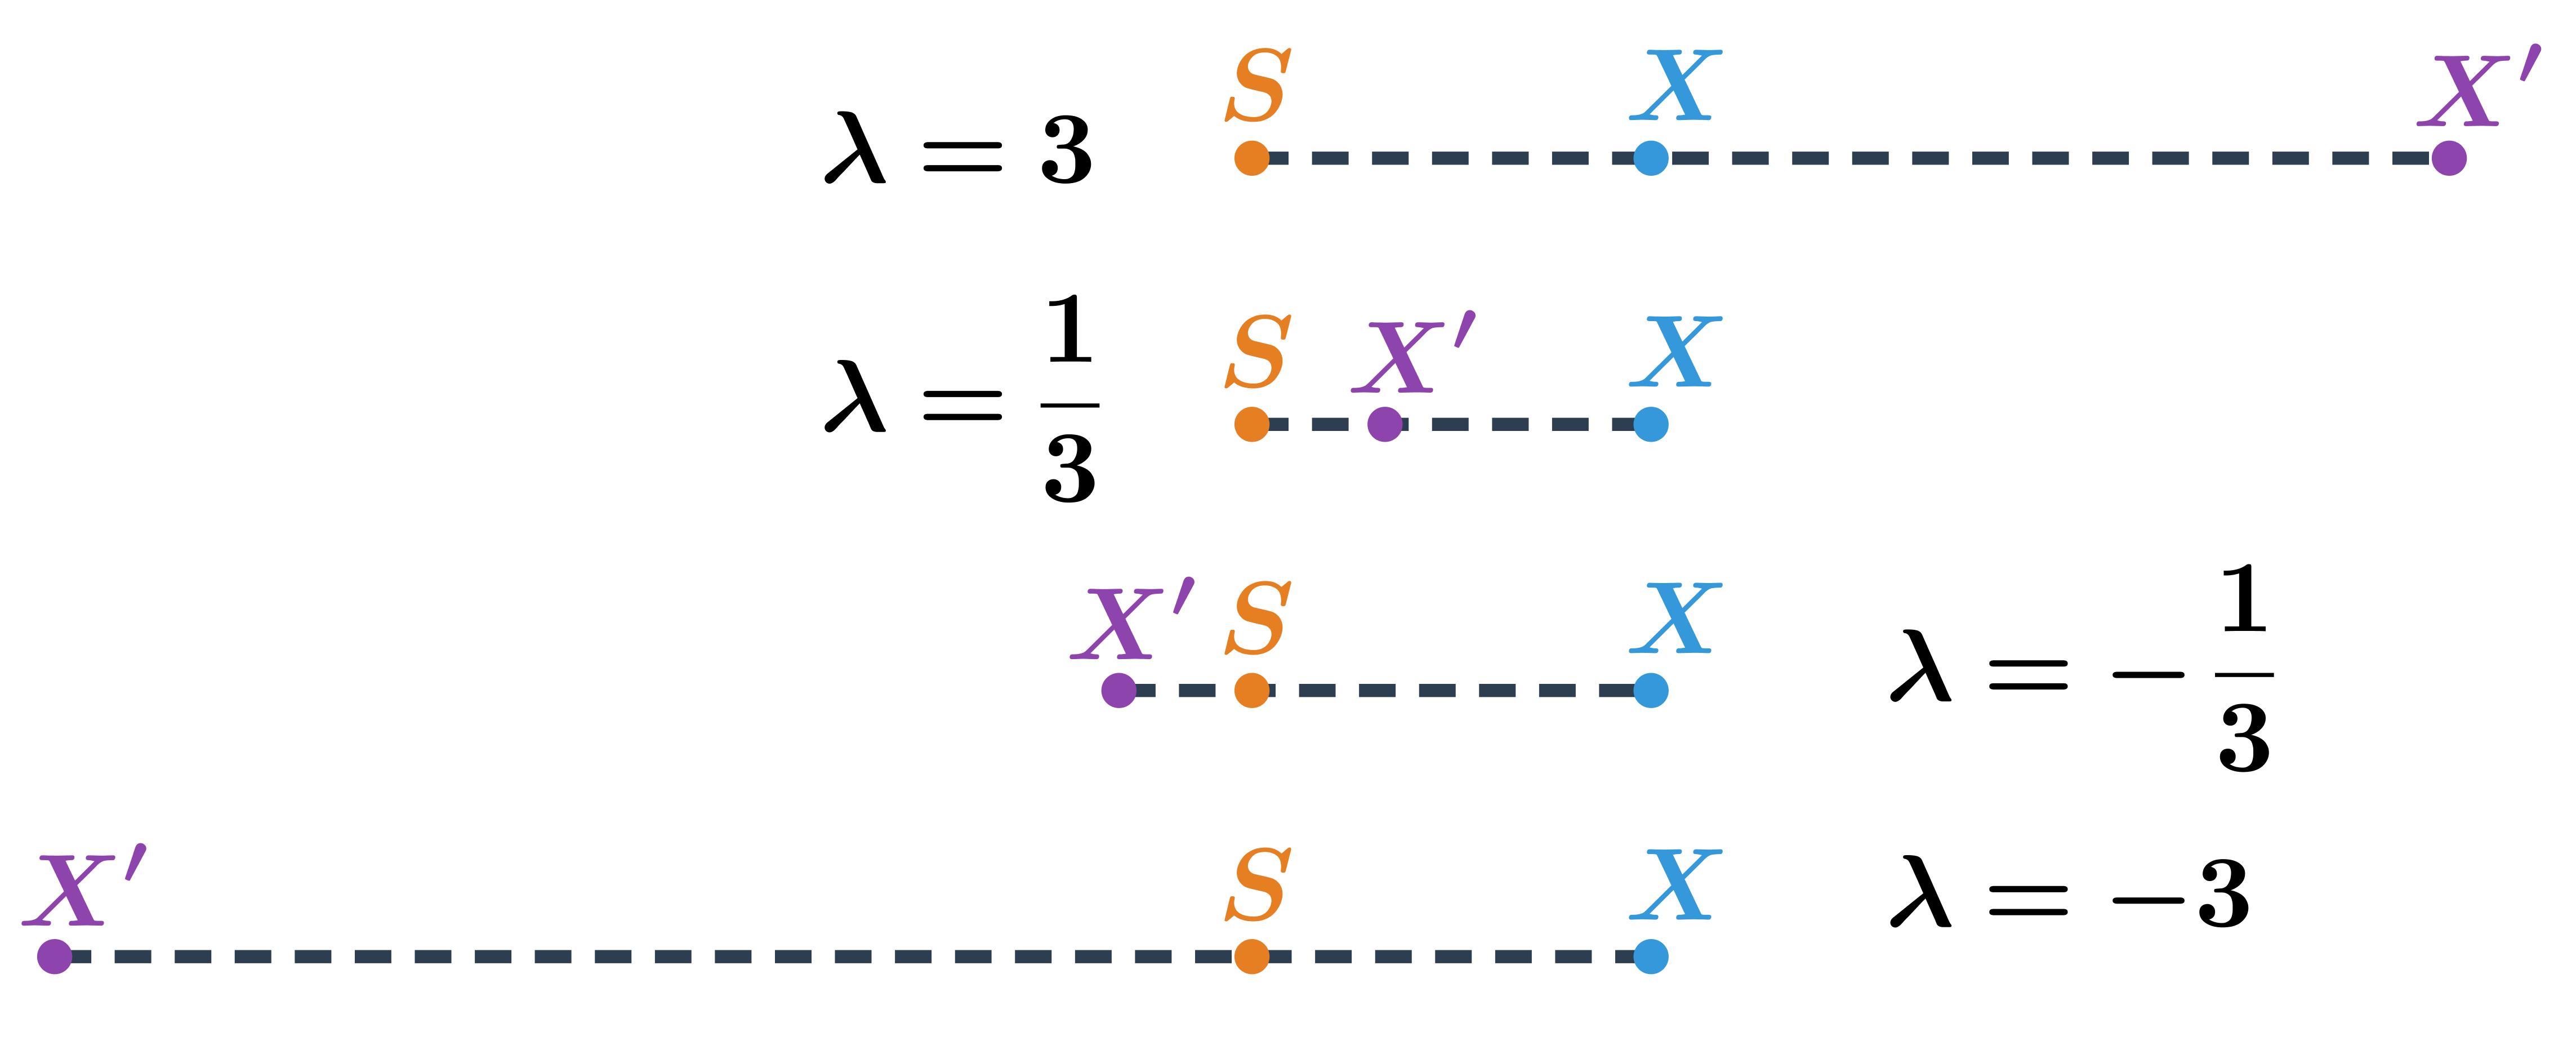
\includegraphics[width=0.5\linewidth]{stejnolehlost.png}
\end{center}
\end{reseni}

\begin{priklad}
Je dána kružnice $k$ a uvnitř ní bod $M$. Sestrojte všechny tětivy této kružnice
procházející bodem $M$, které jsou jím děleny v poměru $3:5.$
\end{priklad}

\begin{reseni}
Označme tětivu jako $XY$ ($X,Y$ jsou tedy na kružnici $k$). Pak $Y$ je obraz
bodu $X$ ve stejnolehlost se středem $M$ a koeficientem $-\frac{5}{3}$. Protože
body $X$ leží na kružnici $k,$ pak bod $Y$ leží na kružnici $k^\prime$ (tj. obraz
kružnice $k$ ve výše popsané stejnolehlosti). Proto je $Y$ průsečík $k\cap k^\prime$.
\end{reseni}

\begin{priklad}
Je dán konvexní úhel $AVB$ a vnitřní bod $M$ tohoto úhlu. Sestrojte kružnici $k,M\in k,$
která se dotýká obou ramen úhlu.
\end{priklad}

\begin{reseni}
Sestrojíme si libovolnou kružnici $k^\prime$, která se dotýká ramen úhlu $AVB$ a pak
ji zobrazíme ve stejnolehlost se středem $V$ a koeficientem $\frac{|VM|}{|VM^\prime|},$
kde $M^\prime$ je průsečík úsečky $VM$ a kružnice $k^\prime$.
\end{reseni}

\begin{priklad}
Je dána přímka $p$, kružnice $k$, která nemá s přímkou $p$ společný bod a bod $A$, který
neleží ani na přímce $p$, ani ve vnitřní oblasti kružnice $k$. Sestrojte trojúhelník
$ABC$ s úhlem $|\sphericalangle BAC|=60^\circ$ tak, aby $B\in p, C \in k, |AC|=2|AB|.$
\end{priklad}

\begin{reseni}
Bod $C$ je obraz bodu $B$ ve složeném zobrazení ze stejnolehlosti se středem v bodě
$A$ a koeficientem 2 a následném otočení o $60^\circ.$ \dots Proto je bod $C$ průsečík
kružnice $k$ a přímky $p^\prime$ získené výše popsaným zobrazením.
\end{reseni}
